\chapter{Observables and Inner Products}
\label{ch:observables}

In this chapter we develop the machinery necessary to get information out of the
wavepackets whose time-evolution we will simulate. An essential part is the computation
of several types of brakets. This will be done numerically by a special, high-order
quadrature rule.


\section{Observables in general}


To compute any observable $O$ we have to form the full braket:

\begin{equation}
  O = \Braket{\Psi | \hat{O} | \Psi}
\end{equation}

which boils down to a multi-dimensional integral. We look at the most general
case and seek to compute:

\begin{equation}
  \Braket{\Psi^\prime | \mathcal{F} | \Psi}
\end{equation}

where the operator $\mathcal{F}$ is a $N \times N$ matrix of scalar functions
$\mathcal{F}_{r,c}(\vec{x})$. The wavepackets $\Psi$ and $\Psi^\prime$ are
assumed to be of inhomogeneous type and can have different parameter sets
$\Pi$ and $\Pi^\prime$. The ansatz is:

\begin{align*}
  \Braket{\Psi^\prime | \mathcal{F} | \Psi} & =
  \Braket{
    \begin{pmatrix}
      \Phi_0^\prime \\ \vdots \\ \Phi_{N-1}^\prime
    \end{pmatrix}
    |
    \begin{pmatrix}
      {}     & \vdots            & {} \\
      \cdots & \mathcal{F}_{r,c} & \cdots \\
      {}     & \vdots            & {}
    \end{pmatrix}
    |
    \begin{pmatrix}
      \Phi_0 \\ \vdots \\ \Phi_{N-1}
    \end{pmatrix}
  } \\
  & =
  \sum_{r=0}^{N-1} \sum_{c=0}^{N-1}
  \Braket{\Phi_r^\prime | \mathcal{F}_{r,c} | \Phi_c} \,.
\end{align*}

We continue by using the definition \eqref{eq:scalar_wavepacket} for the
individual components and resolve:

\begin{align*}
  \Braket{\Phi^\prime_r | \mathcal{F}_{r,c} | \Phi_c} & =
  \Braket{\sum_{\vec{k}\in\mathfrak{K}^\prime_r} \phi^\prime_{\vec{k}}
          | \mathcal{F}_{r,c} |
          \sum_{\vec{l}\in\mathfrak{K}_c} \phi_{\vec{l}}} \\
  & =
  \sum_{\vec{k}\in\mathfrak{K}^\prime_r}
  \sum_{\vec{l}\in\mathfrak{K}_c}
  \Braket{\phi^\prime_{\vec{k}} | \mathcal{F}_{r,c} | \phi_{\vec{l}}}
\end{align*}

where we left out the global phase as well as the coefficients. The last
braket consists of basis functions only and we know that:

\begin{equation*}
  \Braket{\phi^\prime_{\vec{k}} | \mathcal{F}_{r,c} | \phi_{\vec{l}}}
  =
  \idotsint \conj{\phi^\prime_{\vec{k}}(\vec{x})} \mathcal{F}_{r,c}(\vec{x}) \phi_{\vec{l}}(\vec{x}) \mathrm{d}\vec{x} \,.
\end{equation*}

Hence we make a longer detour and examine the computation of any
inner-product like this one before we return to observables.


\section{Inner products}


\subsection{Integrals over basis functions}


In the following we want to compute inner products of the form
$\Braket{\phi_k[\Pi_k]|\phi_l[\Pi_l]}$ with just an identity
in place of $\mathcal{F}_{r,c}$ from above. We abuse the notation
here. The indices $k$ and $l$ are not multi-indices and do not index
the $\phi$ in the corresponding basis set. They are solely used to
discriminate between the bra and the ket, to make clear which
function $\phi$ and parameter set $\Pi$ we speak of. There is no useful
closed form solution to this integral and we have to compute it
numerically by using quadrature. For the derivation of the quadrature
formulae we work with the ground states only and hence $\phi_k = \phi^\prime_{\vec{0}}$
and $\phi_l = \phi_{\vec{0}}$.


\subsection{Quadrature rules}


To compute the integral shown in the last section we use a Gauss-Hermite
quadrature rule of very high order. The properties of this quadrature rule
make it well-suited for our purpose. The quadrature rule $\rho$ consists of
nodes $\gamma$ and weights $\omega$. In the case of Gauss-Hermite quadrature
these values are built to integrate $f(x)$ in:

\begin{equation} \label{eq:gh_integral}
  \int_{\mathbb{R}} e^{-x^2} f(x) \mathrm{d}x \approx \sum_{i=0}^{R-1} \omega_i f(\gamma_i) \,.
\end{equation}

For a quadrature of order $R$ the nodes $\{\gamma_i\}_{i=0}^{R-1}$ are then
given as the roots of the Hermite polynomial $H_R(x)$:

\begin{equation*}
  H_R(x) = (-1)^R e^{x^2} \frac{d^R}{dx^R} e^{-x^2} \,.
\end{equation*}

Of course we do not compute the nodes by finding the roots of these polynomials
as this is inherently unstable. The quadrature weights are then given by:

\begin{equation*}
  \omega_i = \frac{2^{R-1} R! \sqrt{\pi}} {R^2 H_{R-1}^2(\gamma_i)} \,.
\end{equation*}

Since our integrals are not of the form \eqref{eq:gh_integral}
but instead we have:

\begin{equation}
  \int_{\mathbb{R}} g(x) \mathrm{d}x
\end{equation}

where the $\exp(-x^2)$ is built into the function $g(x)$ such that
$g(x) = \exp(-x^2) f(x)$, we have to alter the ansatz. We can not divide
by $\exp(-x^2)$ without getting major numerical instabilities. But we can
modify our quadrature weights to take that factor into account. We define
new quadrature weights $\omega_i^\prime$ as:

\begin{equation*}
  \omega_i^\prime \assign \frac{1}{R \, h_R^2(\gamma_i)}
\end{equation*}

where $h_R$ are the Hermite functions defined as:

\begin{equation*}
  h_R(x) \assign \frac{1}{\sqrt{2^R R! \sqrt{\pi}}} e^{-x^2/2} H_R(x) \,.
\end{equation*}

We can evaluate the Hermite function for any point $x$ by a stable,
recursive scheme. Finally the quadrature rule $\rho$ in use is
given by:

\begin{equation}
  \rho \assign \left\{\left(\gamma_i, \omega_i^\prime\right)\right\}_{i=0}^{R-1}
\end{equation}

for one space dimension. In higher dimensions we build a quadrature
rule $\rho$ by computing the full tensor product of $D$ one-dimensional
quadrature rules $\rho_d$:

\begin{equation}
  \rho \assign \bigotimes_{d=0}^{D-1} \rho_d \,.
\end{equation}

Using the rules $\rho_d$, each of order $R_d$, we get the $D$-dimensional
rule then denoted by:

\begin{equation}
  \rho \assign \left\{ \left( \vec{\gamma}_i, \omega_i \right) \right\}_{i=0}^{R-1}
\end{equation}

with a total number $R = \prod_{d=0}^{D-1} R_d$ of quadrature nodes. The quadrature
nodes $\vec{\gamma}_{\vec{j}} \in \mathbb{R}^D$ are constructed as:

\begin{equation*}
  \vec{\gamma}_{\vec{j}}
  \assign
  \begin{pmatrix}
    \gamma^0_{\vec{j}_0} \\
    \vdots \\
    \gamma^{D-1}_{\vec{j}_{D-1}}
  \end{pmatrix}
\end{equation*}

with $\vec{j} \in [0,R_0-1] \times \cdots \times [0,R_{D-1}-1]$ a multi-index.
Each of the $\gamma^d$ belongs to the one-dimensional rule $\rho_d$. For the
weights $\omega_i$ of $\rho$ we have:

\begin{equation*}
  \omega_{\vec{j}} \assign \prod_{d=0}^{D-1} \omega^d_{\vec{j}_d}
\end{equation*}

and again $\omega^d$ is part of $\rho_d$. Figure \ref{fig:tensor_product_qr}
shows a typical two-dimensional quadrature rule.

\begin{figure}
  \centering
  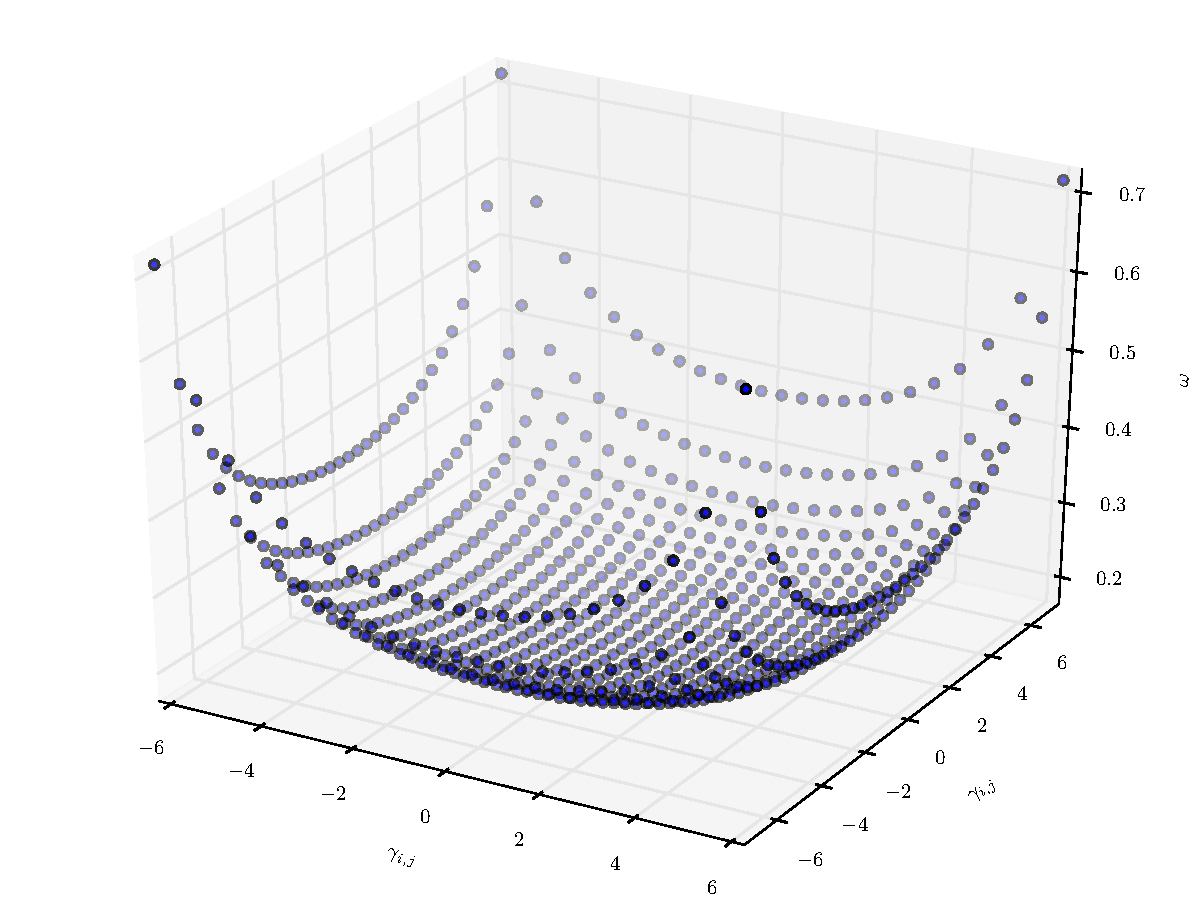
\includegraphics[width=0.8\linewidth]{./fig/tensor_qr.pdf}
  \caption[A two-dimensional quadrature rule]{
    Plot of the nodes $\vec{\gamma}_i$ and weights $\omega_i$ of
    a two-dimensional quadrature rule $\rho$. The rule is build
    from two one-dimensional rules of order $24$ and $32$.
  }
  \label{fig:tensor_product_qr}
\end{figure}


\subsection{Adapting the quadrature}


Since the basis functions are parametrised we have to adapt the quadrature rule
$\{\vec{\gamma_i}, \omega_i\}_i$ to fit best the given situation depending on the
sets $\Pi_k$ and $\Pi_l$. If both functions in the bra and the ket are members of
the same family with $\Pi_k \equiv \Pi_l$ the process is much easier and we will
do this case first. But we will need also the more general case where $\Pi_k \neq \Pi_l$
later. The purpose of this subsection is to find a transformation rule for the quadrature
nodes $\vec{\gamma_i}$ to suit the wavepacket's basis best. The final rule will
be an affine transformation like:

\begin{equation} \label{eq:transformed_qr_nodes}
  \vec{\gamma_i}^\prime = \vec{v} + \mat{A} \vec{\gamma_i}
\end{equation}

where the quadrature node $\vec{\gamma_i} \in \mathbb{R}^D$, the offset vector
$\vec{v} \in \mathbb{R}^D$ and the transformation matrix $\mat{A} \in \mathbb{R}^{D \times D}$.


\subsection{The homogeneous case}


We first threat the homogeneous case of the overlap integral. This case is
much easier as we assume that we have the same wavepacket in the bra as well
as in the ket. Hence the inner-product simplifies to $\Braket{\phi|\phi}$
and we have the same set $\Pi$ of Hagedorn Parameters. This makes combining
the two exponential terms from the definition \eqref{eq:phi0_Dd} into a single one
of the same form much easier.

We concentrate on the exponential parts which dominate the overall shape of the
basis functions and we are interested in the quadratic term only. Essentially we
only need to know where the peak of the Gaussian is and how big the spread is.

\begin{align*}
  \Braket{\phi|\phi} = & \\
  \exp\Bigg( &
      \conj{\frac{i}{2\varepsilon^2} \dotp{\ofs{\vec{x}-\vec{q}}}{\mat{P} \mat{Q}\inv \ofs{\vec{x}-\vec{q}}}
      + \frac{i}{\varepsilon^2} \dotp{\vec{p}}{\ofs{\vec{x}-\vec{q}}}}
      \\
    & + \frac{i}{2\varepsilon^2} \dotp{\ofs{\vec{x}-\vec{q}}}{\mat{P} \mat{Q}\inv \ofs{\vec{x}-\vec{q}}}
      + \frac{i}{\varepsilon^2} \dotp{\vec{p}}{\ofs{\vec{x}-\vec{q}}}
  \Bigg) \\
  = \exp\Bigg( &
      \frac{-i}{2\varepsilon^2} \conj{\dotp{\ofs{\vec{x}-\vec{q}}}{\mat{P} \mat{Q}\inv \ofs{\vec{x}-\vec{q}}}}
      + \frac{-i}{\varepsilon^2} \conj{\dotp{\vec{p}}{\ofs{\vec{x}-\vec{q}}}}
      \\
    & + \frac{i}{2\varepsilon^2} \dotp{\ofs{\vec{x}-\vec{q}}}{\mat{P} \mat{Q}\inv \ofs{\vec{x}-\vec{q}}}
      + \frac{i}{\varepsilon^2} \dotp{\vec{p}}{\ofs{\vec{x}-\vec{q}}}
  \Bigg) \\
  = \exp\Bigg( &
      \frac{-i}{2\varepsilon^2} \dotp{\mat{P} \mat{Q}\inv \ofs{\vec{x}-\vec{q}}}{\ofs{\vec{x}-\vec{q}}}
      + \frac{-i}{\varepsilon^2} \dotp{\ofs{\vec{x}-\vec{q}}}{\vec{p}}
      \\
    & + \frac{i}{2\varepsilon^2} \dotp{\ofs{\vec{x}-\vec{q}}}{\mat{P} \mat{Q}\inv \ofs{\vec{x}-\vec{q}}}
      + \frac{i}{\varepsilon^2} \dotp{\vec{p}}{\ofs{\vec{x}-\vec{q}}}
  \Bigg)
\end{align*}

For the sake of readability we define the matrix:

\begin{equation*}
  \mat{\Gamma} \assign \mat{P} \mat{Q}\inv
\end{equation*}

and continue. From now on we drop the exponential and work on the exponent only.
(The equal signs have to be understood within this laziness.)

\begin{align*}
  & =
    \frac{i}{2\varepsilon^2} \dotp{\ofs{\vec{x}-\vec{q}}}{\mat{\Gamma} \ofs{\vec{x}-\vec{q}}}
  - \frac{i}{2\varepsilon^2} \dotp{\mat{\Gamma} \ofs{\vec{x}-\vec{q}}}{\ofs{\vec{x}-\vec{q}}}
  + \frac{i}{\varepsilon^2} \dotp{\vec{p}}{\ofs{\vec{x}-\vec{q}}}
  - \frac{i}{\varepsilon^2} \dotp{\ofs{\vec{x}-\vec{q}}}{\vec{p}} \\
  & =
    \frac{i}{2\varepsilon^2} \Bigl( \dotp{\ofs{\vec{x}-\vec{q}}}{\mat{\Gamma} \ofs{\vec{x}-\vec{q}}} - \dotp{\mat{\Gamma} \ofs{\vec{x}-\vec{q}}}{\ofs{\vec{x}-\vec{q}}} \Bigr)
  + \frac{i}{\varepsilon^2} \Bigl( \dotp{\vec{p}}{\ofs{\vec{x}-\vec{q}}} - \dotp{\ofs{\vec{x}-\vec{q}}}{\vec{p}} \Bigr)
\end{align*}

The linear terms vanish as the inner-product is symmetric for entirely real arguments.
We then rearrange and combine the brakets:

\begin{align*}
  & =
  \frac{i}{2\varepsilon^2} \Bigl( \dotp{\ofs{\vec{x}-\vec{q}}}{\mat{\Gamma} \ofs{\vec{x}-\vec{q}}} - \dotp{\ofs{\vec{x}-\vec{q}}}{\mat{\Gamma}\H \ofs{\vec{x}-\vec{q}}} \Bigr) \\
  & =
  \frac{i}{2\varepsilon^2} \dotp{\ofs{\vec{x}-\vec{q}}}{\left(\mat{\Gamma} - \mat{\Gamma}\H\right) \ofs{\vec{x}-\vec{q}}} \,.
\end{align*}

Now we are almost done. The term on the last line is of the same form as the
quadratic one in the definition of $\Ket{\phi}$. Hence we succeeded in combining
the Gaussian exponential parts of two wavepackets into a single one.

The only thing left is to simplify the operator $\mat{\Gamma} - \mat{\Gamma}\H$ but this
is not difficult. Recalling the definition of $\mat{\Gamma}$ we get:

\begin{align*}
  \mat{\Gamma} - \mat{\Gamma}\H
  & = \mat{P} \mat{Q}\inv - \left(\mat{P} \mat{Q}\inv\right)\H \\
  & = \mat{P} \mat{Q}\inv - \mat{Q}\Hinv \mat{P}\H \\
  & = \mat{P} \mat{Q}\inv - \left(\mat{P} \mat{Q}\inv\right)\H \,.
\end{align*}

Remembering the second of the two compatibility conditions in \eqref{eq:PQcond_Dd} we get:

\begin{align*}
  \mat{Q}\H \mat{P} - \mat{P}\H \mat{Q} & = 2i \id \\
  \mat{Q}\Hinv \mat{Q}\H \mat{P} - \mat{Q}\Hinv \mat{P}\H \mat{Q} & = 2i \mat{Q}\Hinv \\
  \mat{P} \mat{Q}\inv - \mat{Q}\Hinv \mat{P}\H \mat{Q} \mat{Q}\inv & = 2i \mat{Q}\Hinv \mat{Q}\inv \\
  \mat{P} \mat{Q}\inv - \mat{Q}\Hinv \mat{P}\H & = 2i \mat{Q}\Hinv \mat{Q}\inv \\
  \mat{P} \mat{Q}\inv - \left(\mat{P} \mat{Q}\inv\right)\H & = 2i \left(\mat{Q} \mat{Q}\H\right)\inv
\end{align*}

where we used identities from \cite{P_matrix_book}. Hence:

\begin{equation*}
    \mat{\Gamma} - \mat{\Gamma}\H = 2i \left(\mat{Q} \mat{Q}\H\right)\inv \,.
\end{equation*}

We want the combined wavepacket to look like the following (which is motivated
by the reason that this exactly yields a Gaussian with shift $\vec{q_0}$ and spread $\mat{Q_0}$):

\begin{equation} \label{eq:desired_form}
  \exp{\left( -\frac{1}{\varepsilon^2} \dotp{\ofs{\vec{x}-\vec{q_0}}}{ \mat{Q_0} \ofs{\vec{x}-\vec{q_0}}} + \text{optional junk} \right)}
\end{equation}

where $\vec{q_0} \in \mathbb{R}^D$ and $\mat{Q_0} \in \mathbb{C}^{D \times D}$
are the final parameters to determine.

From above we have:

\begin{align*}
  & \exp\ofs{\frac{i}{2\varepsilon^2} \dotp{\ofs{\vec{x}-\vec{q}}}{\left(\mat{\Gamma} - \mat{\Gamma}\H\right) \ofs{\vec{x}-\vec{q}}}} \\
  & = \exp\ofs{\frac{i}{2\varepsilon^2} \dotp{\ofs{\vec{x}-\vec{q}}}{2i \left(\mat{Q} \mat{Q}\H\right)\inv \ofs{\vec{x}-\vec{q}}}} \\
  & = \exp\ofs{-\frac{1}{\varepsilon^2} \dotp{\ofs{\vec{x}-\vec{q}}}{\left(\mat{Q} \mat{Q}\H\right)\inv \ofs{\vec{x}-\vec{q}}}} \,.
\end{align*}

Therefore we immediately see that we have to set:

\begin{equation} \label{eq:quad_mix_Dd_homog_q0}
\boxed{
  \vec{q_0} = \vec{q}
}
\end{equation}

and:

\begin{equation} \label{eq:quad_mix_Dd_homog_Q0}
\boxed{
  \mat{Q_0} = \ofs{\mat{Q} \mat{Q}\H}\inv
}
\end{equation}

Notice that in the limit of $D \rightarrow 1$ we retrieve the scalar case
presented in \cite{B_bachelor_thesis} where $q_0 \in \mathbb{R}$ and
$Q_0 \in \mathbb{C}$ and:

\begin{align*}
  q_0 & = q \\
  Q_0 & = \ofs{Q \conj{Q}}\inv = \frac{1}{|Q|^2} \,.
\end{align*}


\subsection{The parameter $\mat{Q_S}$}


For the transformation of the quadrature rule $\{\vec{\gamma_i}, \omega_i\}_i$
the values $\mat{Q_0}$ and $\mat{q_0}$ are not enough. We need a parameter
denoted by $\mat{Q_S}$ which is in the one-dimensional case given by:

\begin{equation*}
  Q_S \assign \frac{1}{\sqrt{Q_0}} \,.
\end{equation*}

Therefore our next goal is to find a relation which holds in the $D$-dimensional
case too. We propose in analogy the following formula:

\begin{equation} \label{eq:mixing_Qs}
\boxed{
  \mat{Q_S} \assign \ofs{\sqrt{\mat{Q_0}}}\inv
}
\end{equation}

But we have to find a way to express the root of a matrix in a suitable way. There
is a way to compute almost any scalar function $f\ofs{x}$ for a matrix argument
$\mat{X}$. The trick goes by the similarity transform of $\mat{X}$ and then
computing $f$ on the eigenvalues $\lambda_i$ of $\mat{X}$. But this method relies
on $\mat{X}$ being diagonalisable and $f$ being defined on the whole spectrum of
$\mat{X}$. We will now take a longer but probably cleaner way which in the end
turns out to be not that different.

We are in the homogeneous case and thus $\mat{Q_0} = \ofs{\mat{Q} \mat{Q}\H}\inv$.
Refining the above expression step by step we get:

\begin{align*}
  \mat{Q_S} & \assign \ofs{\sqrt{\mat{Q_0}}}\inv \\
            & = \ofs{\sqrt{\ofs{\mat{Q} \mat{Q}\H}\inv}}\inv \\
            & = \ofs{\sqrt{\ofs{\mat{Q}\H}\inv \mat{Q}\inv}}\inv \\
            & = \ofs{\sqrt{\ofs{\mat{Q}\inv}\H \mat{Q}\inv}}\inv \,.
\end{align*}

If we now define $\mat{X} \assign \mat{Q}\inv$ we get:

\begin{equation}
  \mat{Q_S} \assign \ofs{\sqrt{\mat{X}\H \mat{X}}}\inv \,.
\end{equation}

For a complex square matrix $\mat{A}$ one can define the so called \emph{polar decomposition}
as follows:

\begin{equation*}
  \mat{A} \rassign \mat{U} \mat{P}
\end{equation*}

where $\mat{U}$ is unitary and $\mat{P}$ is a positive-semidefinite Hermitian matrix.
The two factors are given as:

\begin{align*}
  \mat{P} & \assign \sqrt{\mat{A}\H \mat{A}} \\
  \mat{U} & \assign \mat{A} \mat{P}\inv
\end{align*}

with $\mat{P}$ being unique. When looking at $\mat{P}$ we recognise the root
expression from above if we take $\mat{A} \equiv \mat{X} = \mat{Q}\inv$. We have
shown that we can find the matrix $\mat{Q_S}$ by polar decomposition of $\mat{Q}\inv = \mat{U} \mat{P}$.
With this factorisation we can write:

\begin{equation*}
  \mat{Q_S} = \mat{P}\inv = \mat{Q} \mat{U} \,.
\end{equation*}

The remaining question is now how to compute this decomposition of $\mat{Q}\inv$
into $\mat{U}$ and $\mat{P}$. And the answer is quite trivial. One can compute
the polar decomposition of $\mat{A}$ from its \emph{singular value decomposition}.
We write the singular value decomposition as:

\begin{align*}
  \mat{A} \rassign \mat{W} \mat{\Sigma} \mat{V}\H
\end{align*}

where $\mat{W}$ and $\mat{V}$ are two unitary matrices (which in our case are both of the same
size $D \times D$ because we started with a square matrix $\mat{A}$) and $\mat{\Sigma}$ is a
diagonal matrix. Now we can write the two factors $\mat{U}$, $\mat{P}$ of the
polar decomposition of $\mat{A}$ as:

\begin{align*}
  \mat{P} & = \mat{V} \Sigma \mat{V}\H \\
  \mat{U} & = \mat{W} \mat{V}\H \,.
\end{align*}

We obtain the final result for $\mat{Q_S}$ as follows, first we compute the singular
value decomposition of $\mat{Q}\inv$:

\begin{equation*}
  \mat{W} \mat{\Sigma} \mat{V}\H \assign \mat{Q}\inv
\end{equation*}

then we form $\mat{P}\inv$ and simplify the result using the fact that $\mat{V}$ is unitary:

\begin{align*}
  \mat{Q_S} & = \mat{P}\inv \\
      & = \ofs{\mat{V} \mat{\Sigma} \mat{V}\H}\inv \\
      & = \mat{V}\Hinv \mat{\Sigma}\inv \mat{V}\inv \\
      & = \mat{V}\H\H \mat{\Sigma}\inv \mat{V}\H \,.
\end{align*}

At the end of the day we reached our goal and write:

\begin{equation*}
\boxed{
  \mat{Q_S} \assign \mat{V} \mat{\Sigma}\inv \mat{V}\H
}
\end{equation*}

Now we may remember what was mentioned above about computing a function of a matrix.
But instead of the \emph{eigenvalue decomposition} $\mat{T} \mat{\Lambda} \mat{T}\inv$
of $\mat{A}\H \mat{A}$ we used the singular value decomposition. For $\mat{W} \mat{\Sigma} \mat{V}\H = \mat{A}$
recall that $\mat{\Sigma} = \sqrt{\mat{\Lambda}}$ where $\mat{\Lambda}$ is the
diagonal matrix which contains the eigenvalues of $\mat{A}\H \mat{A}$. So what we
did is essentially the same but with less magic. Also notice that the transformation
matrices $\mat{V}$ are unitary hence minimising numerical errors.

To justify this formula further we can show that the reduction $D \rightarrow 1$
to the scalar case yields the correct result. In this case $\mat{Q_0}$ is a $1 \times 1$
matrix as well as $\mat{Q}$. The singular value decomposition $\mat{W} \mat{\Sigma} \mat{V}\H = \mat{A}$
can be computed as:

\begin{align*}
  \mat{W} & \assign \text{eigenvectors}\ofs{\mat{A} \mat{A}\H} \\
  \mat{V} & \assign \text{eigenvectors}\ofs{\mat{A}\H \mat{A}} \\
  \mat{\Sigma} & \assign \sqrt{\text{diagonal}\ofs{\text{eigenvalues}\ofs{\mat{A} \mat{A}\H}}} \,.
\end{align*}

The eigenvector of a $1 \times 1$ matrix is of course just $1$ and the eigenvalue
equals the single entry. Therefore we have:

\begin{equation*}
  \Sigma = \sqrt{\ofs{Q Q\H}\inv} = \sqrt{\frac{1}{\conj{Q}Q}} = \frac{1}{\sqrt{|Q|^2}} = \frac{1}{|Q|}
\end{equation*}

and finally:

\begin{equation*}
  Q_S = \Sigma\inv = |Q| \,.
\end{equation*}

We derived this equation assuming the matrix $\mat{Q_0}$ from the homogeneous mixing
case and also $\mat{Q}$ enters in the singular value decomposition. In the inhomogeneous
case however we cannot apply it because we do not know what to feed into the
singular value decomposition. In that case we have to rely on other techniques
of computing the square root of a matrix. Details about the computation of
matrix square roots can be found in \cite{H_functions_of_matrices}.


\subsection{The inhomogeneous case}


In this section we do the same derivation as in the last one but now in the fully
generalised case where both wavepackets have different parameter sets $\Pi_k$
and $\Pi_l$. We derive the mixing relations for the $D$ dimensional case.

\begin{align*}
  \Braket{\phi_k|\phi_l} = & \\
  \exp\Bigg( &
      \conj{\frac{i}{2\varepsilon^2} \dotp{\ofs{\vec{x}-\vec{q_k}}}{\mat{P_k} \mat{Q_k}\inv \ofs{\vec{x}-\vec{q_k}}}
      + \frac{i}{\varepsilon^2} \dotp{\vec{p_k}}{\ofs{\vec{x}-\vec{q_k}}}}
      \\
    & + \frac{i}{2\varepsilon^2} \dotp{\ofs{\vec{x}-\vec{q_l}}}{\mat{P_l} \mat{Q_l}\inv \ofs{\vec{x}-\vec{q_l}}}
      + \frac{i}{\varepsilon^2} \dotp{\vec{p_l}}{\ofs{\vec{x}-\vec{q_l}}}
  \Bigg) \\
  = \exp\Bigg( &
      \frac{-i}{2\varepsilon^2} \conj{\dotp{\ofs{\vec{x}-\vec{q_k}}}{\mat{P_k} \mat{Q_k}\inv \ofs{\vec{x}-\vec{q_k}}}}
      + \frac{-i}{\varepsilon^2} \conj{\dotp{\vec{p_k}}{\ofs{\vec{x}-\vec{q_k}}}}
      \\
    & + \frac{i}{2\varepsilon^2} \dotp{\ofs{\vec{x}-\vec{q_l}}}{\mat{P_l} \mat{Q_l}\inv \ofs{\vec{x}-\vec{q_l}}}
      + \frac{i}{\varepsilon^2} \dotp{\vec{p_l}}{\ofs{\vec{x}-\vec{q_l}}}
  \Bigg) \\
  = \exp\Bigg( &
      \frac{-i}{2\varepsilon^2} \dotp{\mat{P_k} \mat{Q_k}\inv \ofs{\vec{x}-\vec{q_k}}}{\ofs{\vec{x}-\vec{q_k}}}
      + \frac{-i}{\varepsilon^2} \dotp{\ofs{\vec{x}-\vec{q_k}}}{\vec{p_k}}
      \\
    & + \frac{i}{2\varepsilon^2} \dotp{\ofs{\vec{x}-\vec{q_l}}}{\mat{P_l} \mat{Q_l}\inv \ofs{\vec{x}-\vec{q_l}}}
      + \frac{i}{\varepsilon^2} \dotp{\vec{p_l}}{\ofs{\vec{x}-\vec{q_l}}}
  \Bigg)
\end{align*}

Define the two matrices:

\begin{align*}
  \mat{\Gamma_k} & \assign \mat{P_k} \mat{Q_k}\inv \\
  \mat{\Gamma_l} & \assign \mat{P_l} \mat{Q_l}\inv
\end{align*}

and place them in the above expressions. From this line on we only care about the
argument of the exponential:

\begin{align*}
  & = \frac{i}{2\varepsilon^2} \dotp{\ofs{\vec{x}-\vec{q_l}}}{\mat{\Gamma_l} \ofs{\vec{x}-\vec{q_l}}}
    - \frac{i}{2\varepsilon^2} \dotp{\mat{\Gamma_k} \ofs{\vec{x}-\vec{q_k}}}{\ofs{\vec{x}-\vec{q_k}}}
    + \frac{i}{\varepsilon^2} \dotp{\vec{p_l}}{\ofs{\vec{x}-\vec{q_l}}}
    - \frac{i}{\varepsilon^2} \dotp{\ofs{\vec{x}-\vec{q_k}}}{\vec{p_k}} \\
  & = \frac{i}{2\varepsilon^2} \Bigl(
    \dotp{\ofs{\vec{x}-\vec{q_l}}}{\mat{\Gamma_l} \ofs{\vec{x}-\vec{q_l}}} - \dotp{\mat{\Gamma_k} \ofs{\vec{x}-\vec{q_k}}}{\ofs{\vec{x}-\vec{q_k}}}
    \Bigr) + \frac{i}{\varepsilon^2} \Bigl(
    \dotp{\vec{p_l}}{\ofs{\vec{x}-\vec{q_l}}} - \dotp{\ofs{\vec{x}-\vec{q_k}}}{\vec{p_k}}
    \Bigr) \,.
\end{align*}

This time the linear part won't vanish and we can not drop it. But we can ignore it.
(Be very attentive while reading the formulae as we will ignore more and more junk
terms that are not helpful for reaching our goal.)

\begin{align*}
  & = \frac{i}{2\varepsilon^2} \Bigl(
    \dotp{\ofs{\vec{x}-\vec{q_l}}}{\mat{\Gamma_l} \ofs{\vec{x}-\vec{q_l}}} - \dotp{\ofs{\vec{x}-\vec{q_k}}}{\mat{\Gamma_k}\H \ofs{\vec{x}-\vec{q_k}}}
    \Bigr) \\
\end{align*}

At this stage we can not combine the two inner products as we did in the homogeneous
case. So the only option left is to expand the brakets:

\begin{align*}
  = \frac{i}{2\varepsilon^2} \Bigl(
    &
      \dotp{\vec{x}}{\mat{\Gamma_l} \vec{x}}
      - \dotp{\vec{x}}{\mat{\Gamma_l} \vec{q_l}}
      - \dotp{\vec{q_l}}{\mat{\Gamma_l} \vec{x}}
      + \dotp{\vec{q_l}}{\mat{\Gamma_l} \vec{q_l}} \\
    - & \dotp{\vec{x}}{\mat{\Gamma_k}\H \vec{x}}
      + \dotp{\vec{x}}{\mat{\Gamma_k}\H \vec{q_k}}
      + \dotp{\vec{q_k}}{\mat{\Gamma_k}\H \vec{x}}
      - \dotp{\vec{q_k}}{\mat{\Gamma_k}\H \vec{q_k}}
    \Bigr) \,.
\end{align*}

As a first step towards the goal \eqref{eq:desired_form} we can combine the two terms that are quadratic
in $\vec{x}$.

\begin{align*}
  & = \frac{i}{2\varepsilon^2} \Bigl( \dotp{\vec{x}}{\ofs{\mat{\Gamma_l} - \mat{\Gamma_k}\H} \vec{x}} + \text{junk} \Bigr) \\
\end{align*}

Notice that when we expand the braket in \eqref{eq:desired_form} we get one
that is quadratic in $\vec{x}$ and looks like $\dotp{\vec{x}}{\mat{Q_0} \vec{x}}$. This is essentially
what we wrote on the line above. We just have to find a way to transform the
prefactors. And the way to achieve this goes by taking the imaginary part and
pulling a factor of $\frac{1}{2}$ inside the braket:

\begin{align*}
  & = \frac{i}{2\varepsilon^2} \dotp{\vec{x}}{\ofs{\Re\ofs{\mat{\Gamma_l} - \mat{\Gamma_k}\H}+i\Im\ofs{\mat{\Gamma_l} - \mat{\Gamma_k}\H}} \vec{x}} \\
  & = \underbrace{\frac{i}{2\varepsilon^2} \dotp{\vec{x}}{\Re\ofs{\mat{\Gamma_l} - \mat{\Gamma_k}\H} \vec{x}}}_{\text{junk}}
    + \frac{i}{2\varepsilon^2} \dotp{\vec{x}}{i\Im\ofs{\mat{\Gamma_l} - \mat{\Gamma_k}\H} \vec{x}} \\
  & = -\frac{1}{2\varepsilon^2} \dotp{\vec{x}}{\Im\ofs{\mat{\Gamma_l} - \mat{\Gamma_k}\H} \vec{x}} \\
  & = -\frac{1}{\varepsilon^2} \dotp{\vec{x}}{\frac{1}{2}\Im\ofs{\mat{\Gamma_l} - \mat{\Gamma_k}\H} \vec{x}}
\end{align*}

where we made use of the sesquilinearity in many steps. From the last line and when
we compare the quadratic term to \eqref{eq:desired_form} it is obvious that the
parameter $\mat{Q_0}$ has to be:

\begin{equation} \label{eq:quad_mix_Dd_inhomog_Q0}
\boxed{
  \mat{Q_0} \assign \frac{1}{2}\Im\ofs{\mat{\Gamma_l} - \mat{\Gamma_k}\H}
}
\end{equation}

Now we compute the other parameter $\vec{q_0}$. It turns out that this is more difficult.
We could take a look at the scalar one-dimensional case where the real variable
$q_0$ is of the following form:

\begin{equation*}
  q_0 \assign \frac{\Im\ofs{\Gamma_l q_l - \conj{\Gamma_k}q_k}}{\Im\ofs{\Gamma_l - \conj{\Gamma_k}}} \,.
\end{equation*}

In the multi-dimensional case however we deal with vectors in $\mathbb{R}^D$ and
matrices in $\mathbb{C}^{D \times D}$ thus we have to get rid of the fractions
and write proper inverses. Hence we suggest that in our case the vector $\vec{q_0}$
should look like:

\begin{equation} \label{eq:quad_mix_Dd_inhomog_q0}
\boxed{
  \vec{q_0} \assign \ofs{\Im\ofs{\mat{\Gamma_l} - \mat{\Gamma_k}\H}}\inv \Im\ofs{\mat{\Gamma_l} \vec{q_l} - \mat{\Gamma_k}\H \vec{q_k}}
}
\end{equation}

This expression is also motivated from the fact that $\vec{q_k}$, $\vec{q_l}$ are (column)
vectors and $\mat{\Gamma_k}$, $\mat{\Gamma_l}$ and $\mat{Q_0}$ are square matrices.
Hence $\vec{q_0}$ is a vector as it should be. It is easy to show that these two
formulae reduce to \eqref{eq:quad_mix_Dd_homog_q0} and  \eqref{eq:quad_mix_Dd_homog_Q0} when we
choose $\mat{\Gamma_k} \equiv \mat{\Gamma_l}$. Algorithm \ref{al:mixing_hagedorn_parameters}
implements this general $D$-dimensional mixing of two parameter sets $\Pi_k$ and $\Pi_l$.

% If you are satisfied with this hand-waving
% reasoning you can stop reading here. Otherwise be prepared to very tedious linear algebra.
%
% To begin with we should notice that this expression can be recast as
%
% \begin{equation*}
%   \vec{q_0} = \frac{1}{2} \mat{Q_0}\inv \underbrace{\Im\ofs{\mat{\Gamma_l} \vec{q_l} - \mat{\Gamma_k}\H \vec{q_k}}}_{\vec{\Omega}}
% \end{equation*}
%
% where we called the imaginary part term $\vec{\Omega}$ in the following calculations.
% To show that this expression really is what we search for, we insert this
% into equation \eqref{eq:desired_form} and expand. Then we see that we reproduce
% all terms of \eqref{eq:foo} and additionally some junk.
%
% \begin{align*}
%   & \dotp{\ofs{\vec{x}-\vec{q_0}}}{ \mat{Q_0} \ofs{\vec{x}-\vec{q_0}}} \\
%   & = \dotp{\ofs{\vec{x}- \frac{1}{2}\mat{Q_0}\inv\vec{\Omega}}}{ \mat{Q_0} \ofs{\vec{x}- \frac{1}{2}\mat{Q_0}\inv\vec{\Omega}}} \\
%   & = \dotp{\vec{x}}{ \mat{Q_0} \ofs{\vec{x}- \frac{1}{2}\mat{Q_0}\inv\vec{\Omega}}}
%     - \dotp{\frac{1}{2}\mat{Q_0}\inv\vec{\Omega}}{ \mat{Q_0} \ofs{\vec{x}- \frac{1}{2}\mat{Q_0}\inv\vec{\Omega}}} \\
%   & = \dotp{\vec{x}}{ \mat{Q_0} \vec{x}}
%     - \dotp{\vec{x}}{ \mat{Q_0} \frac{1}{2}\mat{Q_0}\inv\vec{\Omega}}
%     - \dotp{\frac{1}{2}\mat{Q_0}\inv\vec{\Omega}}{ \mat{Q_0} \vec{x}}
%     + \dotp{\frac{1}{2}\mat{Q_0}\inv\vec{\Omega}}{ \mat{Q_0} \frac{1}{2}\mat{Q_0}\inv\vec{\Omega}} \\
%   & = \dotp{\vec{x}}{ \mat{Q_0} \vec{x}}
%     - \frac{1}{2}\dotp{\vec{x}}{ \mat{Q_0} \mat{Q_0}\inv\vec{\Omega}}
%     - \frac{1}{2}\dotp{\mat{Q_0}\inv\vec{\Omega}}{ \mat{Q_0} \vec{x}}
%     + \frac{1}{2}\frac{1}{2}\dotp{\mat{Q_0}\inv\vec{\Omega}}{ \mat{Q_0} \mat{Q_0}\inv\vec{\Omega}} \\
%   & = \dotp{\vec{x}}{ \mat{Q_0} \vec{x}}
%     - \frac{1}{2}\dotp{\vec{x}}{\vec{\Omega}}
%     - \frac{1}{2}\dotp{\mat{Q_0}\inv\vec{\Omega}}{\mat{Q_0} \vec{x}}
%     + \frac{1}{4}\dotp{\mat{Q_0}\inv\vec{\Omega}}{\vec{\Omega}} \\
%   & = \dotp{\vec{x}}{ \mat{Q_0} \vec{x}}
%     - \frac{1}{2}\dotp{\vec{x}}{\vec{\Omega}}
%     - \frac{1}{2}\dotp{\vec{\Omega}}{\vec{x}}
%     + \frac{1}{4}\dotp{\vec{\Omega}}{\mat{Q_0}\inv\vec{\Omega}} \\
% \end{align*}
%
% \marginpar{\boxed{\text{WRONG below here}}}
%
% If we now plug in the term for $\vec{\Omega}$ and defer taking imaginary parts we get
%
% \begin{align*}
%   & = \dotp{\vec{x}}{ \mat{Q_0} \vec{x}}
%     - \frac{1}{2}\dotp{\vec{x}}{\Im\ofs{\mat{\Gamma_l} \vec{q_l} - \mat{\Gamma_k}\H \vec{q_k}}}
%     - \frac{1}{2}\dotp{\Im\ofs{\mat{\Gamma_l} \vec{q_l} - \mat{\Gamma_k}\H \vec{q_k}}}{\vec{x}}
%     + \frac{1}{4}\dotp{\Im\ofs{\mat{\Gamma_l} \vec{q_l} - \mat{\Gamma_k}\H \vec{q_k}}}{\mat{Q_0}\inv\Im\ofs{\mat{\Gamma_l} \vec{q_l} - \mat{\Gamma_k}\H \vec{q_k}}} \\
%   & = \dotp{\vec{x}}{ \mat{Q_0} \vec{x}}
%     - \frac{1}{2}\Im\dotp{\vec{x}}{\mat{\Gamma_l} \vec{q_l} - \mat{\Gamma_k}\H \vec{q_k}}
%     - \frac{1}{2}\Im\dotp{\ofs{\mat{\Gamma_l} \vec{q_l} - \mat{\Gamma_k}\H \vec{q_k}}}{\vec{x}}
%     + \frac{1}{4}\Im\dotp{\ofs{\mat{\Gamma_l} \vec{q_l} - \mat{\Gamma_k}\H \vec{q_k}}}{\mat{Q_0}\inv\ofs{\mat{\Gamma_l} \vec{q_l} - \mat{\Gamma_k}\H \vec{q_k}}} \\
%   & = \Im\ofs{ \dotp{\vec{x}}{ \mat{Q_0} \vec{x}}
%     - \frac{1}{2}\dotp{\vec{x}}{\mat{\Gamma_l} \vec{q_l} - \mat{\Gamma_k}\H \vec{q_k}}
%     - \frac{1}{2}\dotp{\ofs{\mat{\Gamma_l} \vec{q_l} - \mat{\Gamma_k}\H \vec{q_k}}}{\vec{x}}
%     + \frac{1}{4}\dotp{\ofs{\mat{\Gamma_l} \vec{q_l} - \mat{\Gamma_k}\H \vec{q_k}}}{\mat{Q_0}\inv\ofs{\mat{\Gamma_l} \vec{q_l} - \mat{\Gamma_k}\H \vec{q_k}}} } \\
% \end{align*}
%
% Once more we expand the inner products and get a bunch of terms
%
% \begin{align*}
%   & = \Im\Bigl( \dotp{\vec{x}}{ \mat{Q_0} \vec{x}}
%     - \frac{1}{2}\dotp{\vec{x}}{\mat{\Gamma_l} \vec{q_l}} + \frac{1}{2}\dotp{\vec{x}}{\mat{\Gamma_k}\H \vec{q_k}}
%     - \frac{1}{2}\dotp{\mat{\Gamma_l} \vec{q_l}}{\vec{x}} + \frac{1}{2}\dotp{\mat{\Gamma_k}\H \vec{q_k}}{\vec{x}} \\
%   & + \frac{1}{4}\dotp{\mat{\Gamma_l} \vec{q_l}}{\mat{Q_0}\inv\mat{\Gamma_l} \vec{q_l}}
%     - \frac{1}{4}\dotp{\mat{\Gamma_l} \vec{q_l}}{\mat{Q_0}\inv\mat{\Gamma_k}\H \vec{q_k}}
%     - \frac{1}{4}\dotp{\mat{\Gamma_k}\H \vec{q_k}}{\mat{Q_0}\inv\mat{\Gamma_l} \vec{q_l}}
%     + \frac{1}{4}\dotp{\mat{\Gamma_k}\H \vec{q_k}}{\mat{Q_0}\inv\mat{\Gamma_k}\H \vec{q_k}} \Bigr) \\
% \end{align*}
%
% Now we can use the definition of $\mat{Q_0}$ and plug it in here.
%
% Have fun \ldots

\begin{algorithm}
\caption{Mixing two sets $\Pi_r$ and $\Pi_c$ of Hagedorn parameters}
\label{al:mixing_hagedorn_parameters}
\begin{algorithmic}
  \REQUIRE Two sets $\Pi_r$ and $\Pi_c$ of Hagedorn parameters
  \STATE // Apply the mixing formula  \eqref{eq:quad_mix_Dd_inhomog_q0} and \eqref{eq:quad_mix_Dd_inhomog_Q0} to the parameters
  \STATE $\mat{\Gamma_r} \assign \mat{P_r} \mat{Q_r}\inv$
  \STATE $\mat{\Gamma_c} \assign \mat{P_c} \mat{Q_c}\inv$
  \STATE $\mat{\Gamma} \assign \Im \left(\mat{\Gamma_c} - \mat{\Gamma_r}\H\right)$
  \STATE $\vec{g} \assign \Im \left(\mat{\Gamma_c} \vec{q_c} - \mat{\Gamma_r}\H \vec{q_r}\right)$
  \STATE $\vec{q_0} \assign \mat{\Gamma}\inv \vec{q}$
  \STATE $\mat{Q_0} \assign \frac{1}{2} \mat{\Gamma}$
  \STATE // Apply the formula \eqref{eq:mixing_Qs}
  \STATE $\mat{Q_S} \assign \left(\sqrt{\mat{Q_0}}\right)\inv$
  \RETURN $\mat{q_0}$ and $\mat{Q_S}$
\end{algorithmic}
\end{algorithm}


\subsection{Quadrature applied}


After we discussed in details the transformation of the quadrature nodes in the
last section we now look at the final quadrature rule. It's not really difficult,
but it's good to write down all the details at least once. First we transform the
quadrature nodes by \eqref{eq:transformed_qr_nodes} giving:

\begin{equation} \label{eq:transform_qr_nodes}
  \vec{\gamma_i}^\prime = \vec{q_0} + \varepsilon \mat{Q_S} \vec{\gamma_i} \,.
\end{equation}

Then we carry out the quadrature for computing the braket:

\begin{equation}
\boxed{
\begin{split}
  \Braket{\phi_k | f | \phi_l}
  \approx
  \varepsilon^D \cdot |\det(\mat{Q_S})| \cdot \sum_{r=0}^{R-1} \conj{\phi_k\ofs{\vec{\gamma_r}^\prime}}
  \cdot f\ofs{\vec{\gamma_r}^\prime} \cdot \phi_l\ofs{\vec{\gamma_r}^\prime} \cdot \omega_r
\end{split}
}
\end{equation}

where the two $\phi$ in general belong to the different families. But if they really
have the same parameter set $\Pi$ then we can simplify this formula slightly. The
trick is that we omit a prefactor of $\frac{1}{\sqrt{\det(\mat{Q})}}$ when evaluating
$\phi\ofs{\vec{\gamma_r}^\prime}$. Because we have two times this evaluation both
prefactors accumulate to $\frac{1}{\det(\mat{Q})}$. In the case of a single family
we have\footnote{
This is in principle a simple but not necessarily obvious computation.
We use several fundamental properties of the determinant.

\begin{equation*}
\begin{split}
  \det\left(\mat{Q_s}\right)
  = \det\left(\left(\sqrt{\mat{Q_0}}\right)\inv\right)
  = \frac{1}{\det\left(\sqrt{\mat{Q_0}}\right)}
  = \frac{1}{\det\left(\sqrt{\left(\mat{Q}\mat{Q}\H\right)\inv}\right)}
  = \frac{1}{\sqrt{\det\left(\left(\mat{Q}\mat{Q}\H\right)\inv\right)}} \\
  = \frac{1}{\sqrt{\frac{1}{\det\left(\mat{Q}\mat{Q}\H\right)}}}
  = \frac{1}{\sqrt{\frac{1}{\det\mat{Q}\det\mat{Q}\H}}}
  = \sqrt{\det\mat{Q}\det\mat{Q}\H}
  = \sqrt{\det\mat{Q}\conj{\det\mat{Q}}}
\end{split}
\end{equation*}
Let $\det\mat{Q}$ be a complex number $z$. Then we get:
\begin{equation*}
  \sqrt{\det\mat{Q}\conj{\det\mat{Q}}}
  = \sqrt{z\conj{z}}
  = \sqrt{|z|^2} = |z| = |\det\mat{Q}|
\end{equation*}

When taking square roots one has to take into account branch cuts of the complex
plane. This is exactly the reason why we try hard to circumvent this computation at all
by omitting the prefactor $\frac{1}{\det\mat{Q}}$ when evaluating the functions $\phi$.
} $\det(\mat{Q_S}) = |\det(\mat{Q})|$ hence the $|\det(\mat{Q_S})|$ outside the
sum cancels nicely with these prefactors. And the above formula becomes:

\begin{equation}
\boxed{
\begin{split}
  \Braket{\phi | f | \phi}
  \approx
  \varepsilon^D \cdot \sum_{r=0}^{R-1} \conj{\phi\ofs{\vec{\gamma_r}^\prime}} \cdot f\ofs{\vec{\gamma_r}^\prime} \cdot \phi\ofs{\vec{\gamma_r}^\prime} \cdot \omega_r
\end{split}
}
\end{equation}


\section{Matrix elements}


Given a scalar function $f(\vec{x})$ and two sets $\left\{\phi_{\vec{k}}\right\}_{\vec{k}\in\mathfrak{K}}$
and $\left\{\phi^\prime_{\vec{l}}\right\}_{\vec{l}\in\mathfrak{K}^\prime}$ of basis functions.
These functions depend as usual on their parameter sets like $\phi\left[\Pi\right]$ and $\phi\left[\Pi^\prime\right]$.
In the general case both parameter sets will be different. We now try to compute
\emph{matrix elements} like this one:

\begin{equation}
  \mat{F}_{\mu_{\mathfrak{K}}(\vec{k}),\mu_{\mathfrak{K}^\prime}(\vec{l})}
  \assign
  \Braket{ \phi_{\vec{k}}\left[\Pi\right] | f | \phi_{\vec{l}}\left[\Pi^\prime\right] } \,.
\end{equation}

We assumed that $\vec{k} \in \mathfrak{K}$ and $\vec{l} \in \mathfrak{K}^\prime$.
The matrix $\mat{F}$ we can build out of these elements is of the following form:

\begin{equation}
  \mat{F} \assign
  \begin{pmatrix}
    {}     & \vdots                                                                                & {} \\
    \cdots & \Braket{ \phi_{\vec{k}}\left[\Pi\right] | f | \phi_{\vec{l}}\left[\Pi^\prime\right] } & \cdots \\
    {}     & \vdots                                                                                & {}
  \end{pmatrix}
\end{equation}

and has size $|\mathfrak{K}| \times |\mathfrak{K}^\prime|$. The order of the entries
is given by the linearisation mappings $\mu_{\mathfrak{K}}$ and $\mu_{\mathfrak{K}^\prime}$.

\begin{algorithm}
\caption{Build the matrix $\mat{F}$ of matrix elements of $f$}
\label{al:build_matrix}
\begin{algorithmic}
  \REQUIRE Two sets $\Phi \assign \left\{\phi_{\vec{k}}\right\}_{\vec{k}\in\mathfrak{K}}$ and
                    $\Phi^\prime \assign \left\{\phi^\prime_{\vec{l}}\right\}_{\vec{l}\in\mathfrak{K}^\prime}$ of basis functions
  \REQUIRE The parameter sets  $\Pi$ and $\Pi^\prime$
  \REQUIRE The basis shapes $\mathfrak{K}$ and $\mathfrak{K}^\prime$
  \REQUIRE A scalar-valued function $f(\vec{x})$
  \REQUIRE A quadrature rule $(\vec{\gamma}_j, \omega_j)$ with $R$ node-weight pairs
  \STATE // Initialise $\mat{F}$ as the zero-matrix
  \STATE $\mat{F} \in \mathbb{C}^{|\mathfrak{K}| \times |\mathfrak{K}^\prime|}, \quad \mathbf{F} \assign \mathbf{0}$
  \STATE // Apply the mixing formula from procedure \ref{al:mixing_hagedorn_parameters} to the parameters
  \STATE $\vec{q_0}, \mat{Q_S} \assign \mathbf{mix\_parameters}(\Pi, \Pi^\prime)$
  \STATE // Transform the quadrature nodes according to \eqref{eq:transform_qr_nodes}
  \STATE $\vec{\gamma}_j^\prime = \vec{q_0} + \varepsilon \, \mat{Q_S} \, \vec{\gamma}_j \quad j = 0, \ldots R-1$
  \STATE // Evaluate the basis functions of both $\Phi$ with algorithm \ref{al:eval_phi_basis}
  \STATE $\mat{B} \assign \mathbf{evaluate\_basis\_at}[\Phi]\left(\left(\vec{\gamma}_0^\prime, \ldots, \vec{\gamma}_{R-1}^\prime\right)\right)$
  \STATE $\mat{B^\prime} \assign \mathbf{evaluate\_basis\_at}[\Phi^\prime]\left(\left(\vec{\gamma}_0^\prime, \ldots, \vec{\gamma}_{R-1}^\prime\right)\right)$
  \STATE // Evaluate the function $f$ for all quadrature nodes $\vec{\gamma}_j$
  \STATE $\left(v_0, \ldots, v_{R-1}\right) \assign f\ofs{\left(\vec{\gamma}_0^\prime, \ldots, \vec{\gamma}_{R-1}^\prime\right)}$
  \STATE // Iterate over all $R$ quadrature pairs $\left(\vec{\gamma}^\prime_j, \omega_j\right)$
  \FOR{$j = 0$ \TO $j = R-1$}
    \STATE $\mat{F} \assign \mat{F} + \varepsilon^D \, v_{j} \, \omega_j \, \conj{\mat{B}[:,j]} \mat{B^\prime}[:,j]\T$
  \ENDFOR
  \RETURN $\mat{F}$
\end{algorithmic}
\end{algorithm}

A generalisation of this algorithm is given in chapter \ref{ch:wavepacket_propagation} by algorithms
\ref{al:build_block_matrix_homog} and \ref{al:build_block_matrix_inhomog}. The basic principle is the
same. Instead of a scalar function $f$ we have a matrix $\mathcal{F}$ full of scalar functions $f_{r,c}$.
The packets are then vector-valued wavepackets of homogeneous or inhomogeneous kind. Their number
of components obviously has to match the shape of $\mathcal{F}$.

The matrix $\mat{F}$ is also used to compute the braket $\Braket{\Phi|f|\Phi^\prime}$
efficiently as shown in algorithm \ref{al:efficient_computation_phi}.

\begin{algorithm}
\caption{Efficient computation of $\Braket{\Phi| f |\Phi^\prime}$}
\label{al:efficient_computation_phi}
\begin{algorithmic}
  \REQUIRE Two scalar wavepackets $\Phi$ and $\Phi^\prime$
  \REQUIRE The basis shapes $\mathfrak{K}$ and $\mathfrak{K}^\prime$ with corresponding mappings $\mu$
  \REQUIRE The scalar function $f\ofs{x}$
  \STATE // Build the matrix $\mat{F}$ by algorithm \ref{al:build_matrix}
  \STATE $\mat{F} \assign \mathbf{build\_block\_matrix}(\Phi, \Phi^\prime, f)$
  \STATE // Stack the coefficients $\{c_{\vec{k}}\}_{\vec{k}\in\mathfrak{K}}$ and $\{c^\prime_{\vec{l}}\}_{\vec{l}\in\mathfrak{K}^\prime}$ into vectors
  \STATE $\vec{c} \assign \left(c_{\mu_{\mathfrak{K}}(\vec{0})} \cdots c_{\mu_{\mathfrak{K}}(\vec{k})} \cdots \right)\T$
  \STATE $\vec{c}^\prime \assign \left(c^\prime_{\mu_{\mathfrak{K}}^\prime(\vec{0})} \cdots c^\prime_{\mu_{\mathfrak{K}}^\prime(\vec{l})} \cdots \right)\T$
  \STATE // Multiply by the coefficient vectors
  \STATE $I \assign \vec{c}\H \mat{F} \vec{c}^\prime$
  \STATE // In case $\Pi \neq \Pi^\prime$ add the global phase
  \STATE $\pi \assign \exp\ofs{\frac{i}{\varepsilon^2}\left(S^\prime - \conj{S}\right)}$
  \RETURN $\pi \, I$
\end{algorithmic}
\end{algorithm}

Concluding this section we make an artificial example. Assume we have a wavepacket
$\Ket{\Psi}$ with one single component $\Phi$. Set the parameters to:

\begin{equation*}
  \vec{q}  =
  \begin{pmatrix}
    3.5 \\ -6.5 \\ 1.2
  \end{pmatrix}
  \quad
  \vec{p} =
  \begin{pmatrix}
   -0.5 \\ -2 \\ 3.4
  \end{pmatrix}
  \quad
  \mat{Q} = \id
  \quad
  \mat{P} = i \id
  \quad
  S = 0
\end{equation*}

and take $\varepsilon = 0.9$. We use a $3 \times 3 \times 3$ hypercubic basis shape
$\mathfrak{K}$ and set $c_{1,2,0} = 1$ and all other coefficients to zero. Next we
compute matrix elements
$\mat{F}_{\mu(\vec{k}), \mu(\vec{l})} = \Braket{\phi_{\vec{k}} | f | \phi_{\vec{k}}}$ for $\vec{k}, \vec{l} \in \mathfrak{K}$
by algorithm \ref{al:build_matrix} (or one of the algorithms \ref{al:build_block_matrix_homog} or \ref{al:build_block_matrix_inhomog}).
The results for different functions $f$ are shown in figure \ref{fig:matrix_elements_example1} and \ref{fig:matrix_elements_example2}.

\begin{figure}
  \centering
  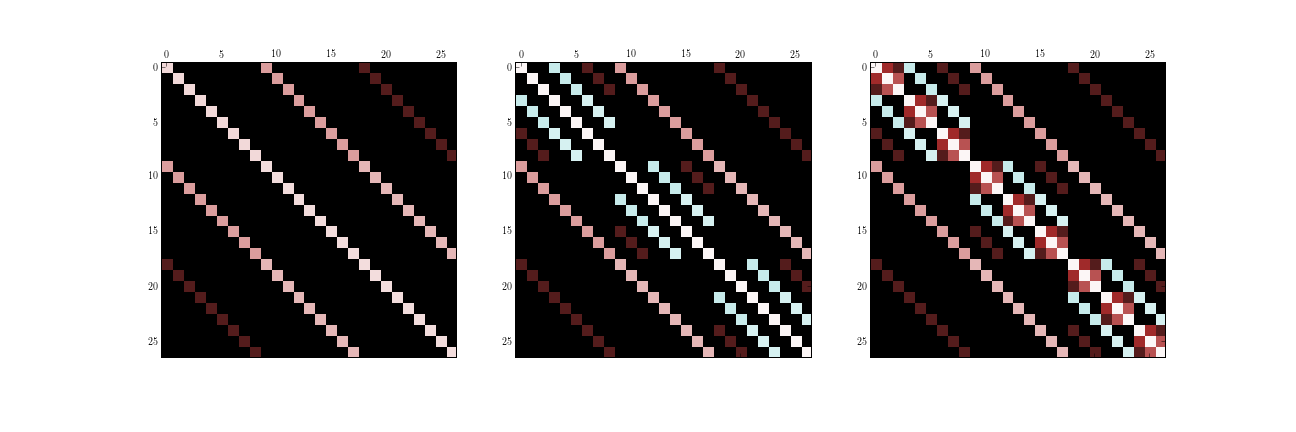
\includegraphics[width=\linewidth]{./fig/matrix_elements_1.png}
  \caption[Matrix elements example 1]{
  The plots show the matrices $\mat{F}$ consisting of the matrix elements $\Braket{\phi_{\vec{k}} | V | \phi_{\vec{l}}}$
  for $V = \frac{1}{2} x^2$ (left), $V = \frac{1}{2} \left(x^2 + y^2\right)$ (middle)
  and $V = \frac{1}{2} \left(x^2 + y^2 + z^2\right)$ (right). For an explanation of the colours, see appendix \ref{ch:color_code}.}
  \label{fig:matrix_elements_example1}
\end{figure}


\begin{figure}
  \centering
  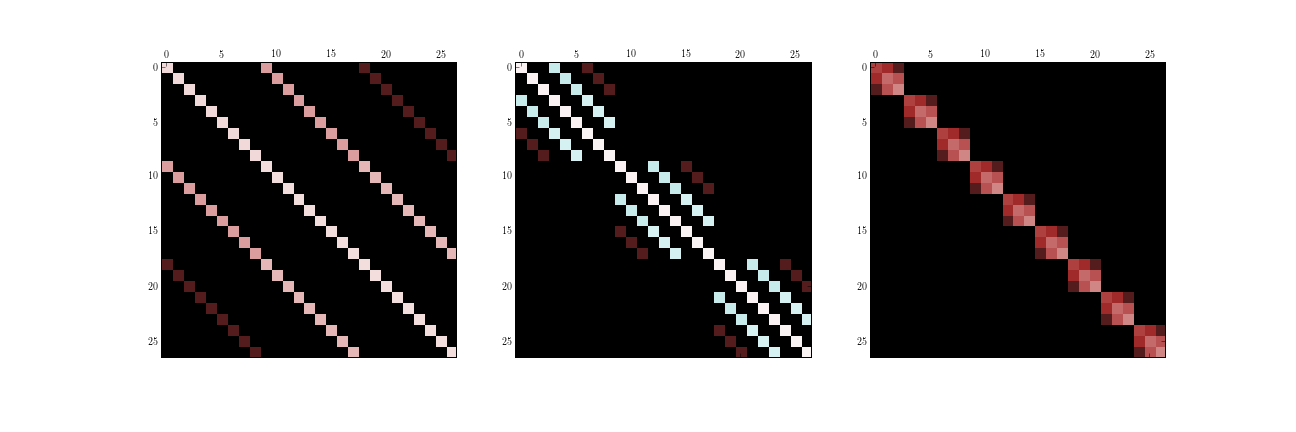
\includegraphics[width=\linewidth]{./fig/matrix_elements_2.png}
  \caption[Matrix elements example 2]{
  The plots show the matrices $\mat{F}$ consisting of the matrix elements $\Braket{\phi_{\vec{k}} | V | \phi_{\vec{l}}}$
  for $V = \frac{1}{2} x^2$ (left), $V = \frac{1}{2} y^2$ (middle)
  and $V = \frac{1}{2} z^2$ (right). For an explanation of the colours, see appendix \ref{ch:color_code}.}
  \label{fig:matrix_elements_example2}
\end{figure}

The block structures in the plots are due to the linearisation mapping $\mu_{\mathfrak{K}}$
and the dependence of $V$ on the variables $x$, $y$ and $z$.


\section{Computing norms of wavepackets}


In the following we want to compute the norm of a wavepacket $\Ket{\Psi}$.
This is the most simple observable or braket where the operator in between
the bra and the ket is just an identity. We start with:

\begin{align*}
  \|\Psi\|^2_{L^2} & = \Braket{\Psi | \Psi} \\
                   & = \sum_{i=0}^{N-1} \Braket{\Phi_i | \Phi_i} \\
                   & = \sum_{i=0}^{N-1} \| \Phi_i \|^2_{L^2} \,.
\end{align*}

Obviously the squared norm of the vector valued wavepacket is the sum of the
squared norms of its components. This is a pattern we will find several times more
when computing observables. In the general case however, the components may get
mixed up by the operator in the middle. Let's continue with calculating the norms
of an individual component which can be considered as a scalar wavepacket. Therefore
we also drop the index $i$ from above.

\begin{align*}
  \Braket{\Phi[\Pi] | \Phi[\Pi]} & = \Braket{ \exp\left(\frac{i S}{\varepsilon^2}\right)
                                              \sum_{\vec{k}\in\mathfrak{K}} c_{\vec{k}} \phi_{\vec{k}}[\Pi](\vec{x})
                                              |
                                              \exp\left(\frac{i S}{\varepsilon^2}\right)
                                              \sum_{\vec{l}\in\mathfrak{K}} c_{\vec{l}} \phi_{\vec{l}}[\Pi](\vec{x})
                                              } \\
  & = \exp\left(\frac{-i S}{\varepsilon^2}\right)\exp\left(\frac{i S}{\varepsilon^2}\right)
      \Braket{ \sum_{\vec{k}\in\mathfrak{K}} c_{\vec{k}} \phi_{\vec{k}}[\Pi](\vec{x})
               |
               \sum_{\vec{l}\in\mathfrak{K}} c_{\vec{l}} \phi_{\vec{l}}[\Pi](\vec{x})
             } \\
\intertext{The global phase cancels here and we get:}
  & = \sum_{\vec{k}\in\mathfrak{K}} \conj{c_{\vec{k}}} \sum_{\vec{l}\in\mathfrak{K}} c_{\vec{l}}
      \Braket{ \phi_{\vec{k}}[\Pi](\vec{x}) | \phi_{\vec{l}}[\Pi](\vec{x}) } \,.
\end{align*}

Now we can exploit the orthonormality condition $\Braket{ \phi_{\vec{k}} | \phi_{\vec{l}} } = \kron{\vec{k},\vec{l}}$
of the basis functions and arrive at:

\begin{equation}
  \|\Phi\|^2_{L^2} = \Braket{\Phi[\Pi] | \Phi[\Pi]} = \sum_{\vec{k}\in\mathfrak{K}} \conj{c_{\vec{k}}} c_{\vec{k}}
                   = \sum_{\vec{k}\in\mathfrak{K}} |c_{\vec{k}}|^2 \,.
\end{equation}


\section{Computing overlap integrals of wavepackets}


If we wanted to compute \emph{overlap integrals} between scalar wavepackets, then
the procedure is very similar but allows for less simplifications. Notice that
now the parameter set $\Pi$ of $\Phi[\Pi]$ can be and in general will be different.
To distinguish them we use $\Pi$ and $\Pi^\prime$.

\begin{align*}
  \Braket{\Phi[\Pi] | \Phi^\prime[\Pi^\prime]}
  & = \Braket{ \exp\left(\frac{i S}{\varepsilon^2}\right)
               \sum_{\vec{k}\in\mathfrak{K}} c_{\vec{k}} \phi_{\vec{k}}[\Pi](\vec{x})
               |
               \exp\left(\frac{i S^\prime}{\varepsilon^2}\right)
               \sum_{\vec{l}\in\mathfrak{K^\prime}} c^\prime_{\vec{l}} \phi_{\vec{l}}[\Pi^\prime](\vec{x})
              } \\
  & = \exp\left(\frac{-i S}{\varepsilon^2}\right)\exp\left(\frac{i S^\prime}{\varepsilon^2}\right)
      \Braket{ \sum_{\vec{k}\in\mathfrak{K}} c_{\vec{k}} \phi_{\vec{k}}[\Pi](\vec{x})
               |
               \sum_{\vec{l}\in\mathfrak{K^\prime}} c^\prime_{\vec{l}} \phi_{\vec{l}}[\Pi^\prime](\vec{x})
             } \\
\intertext{The global phase does not cancel here and we get:}
  & = \exp\left(\frac{-i S}{\varepsilon^2}\right)\exp\left(\frac{i S^\prime}{\varepsilon^2}\right)
      \sum_{\vec{k}\in\mathfrak{K}} \conj{c_{\vec{k}}} \sum_{\vec{l}\in\mathfrak{K^\prime}} c^\prime_{\vec{l}}
      \Braket{ \phi_{\vec{k}}[\Pi](\vec{x}) | \phi_{\vec{l}}[\Pi^\prime](\vec{x}) } \,.
\end{align*}

At the end of the day we get the following formula for the overlap of two scalar wavepackets:

\begin{equation}
  \Braket{\Phi[\Pi] | \Phi^\prime[\Pi^\prime]}
  =
  \exp\left(\frac{i}{\varepsilon^2}(S^\prime - S)\right)
  \sum_{\vec{k}\in\mathfrak{K}} \sum_{\vec{l}\in\mathfrak{K^\prime}} \conj{c_{\vec{k}}} c^\prime_{\vec{l}}
  \Braket{ \phi_{\vec{k}}[\Pi] | \phi_{\vec{l}}[\Pi^\prime] } \,.
\end{equation}

This is the most general formula for overlap integrals (which includes computation of norms).
We allowed for different Hagedorn parameter sets $\Pi$ and $\Pi^\prime$ as well as different
basis shapes $\mathfrak{K}$ and $\mathfrak{K}^\prime$. Hereby we conclude this section and
continue with the computation of energies in the next one.


\section{Computing energies of wavepackets}


To compute the energies of a wavepacket we start with the full Hamiltonian $\mat{H} = \mat{T} + \mat{V}(\vec{x})$.
Then the total energy of $\Ket{\Psi}$ is given by:

\begin{equation}
  E_{\text{total}} = \Braket{\Psi | \mat{H} | \Psi} \,.
\end{equation}

Next we split this braket into the kinetic energy and the potential energy contribution:

\begin{align*}
  E_{\text{total}} & = \Braket{\Psi | \mat{H} | \Psi}
                   & = \Braket{\Psi | \mat{T} | \Psi} + \Braket{\Psi | \mat{V}(\vec{x}) | \Psi}
                     = E_{\text{kinetic}} + E_{\text{potential}} \,.
\end{align*}

\subsection{Potential energy}

We start by computing the potential energy explicitly. Recall the definition of the
potential given in equation \eqref{eq:potential_matrix}. Plugging this matrix
$\mat{V}(\vec{x})$ into the braket above we get:

\begin{align*}
  E_{\text{potential}}
  & = \Braket{\Psi | \mat{V}(\vec{x}) | \Psi} \\
  & = \Braket{
    \begin{pmatrix}
      \Phi_0(\vec{x}) \\
      \vdots \\
      \Phi_{N-1}(\vec{x}) \\
    \end{pmatrix}
    |
    \begin{pmatrix}
      v_{0,0}(\vec{x})   & \cdots & v_{0,N-1}(\vec{x}) \\
      \vdots             &        & \vdots \\
      v_{N-1,0}(\vec{x}) & \cdots & v_{N-1,N-1}(\vec{x})
    \end{pmatrix}
    \begin{pmatrix}
      \Phi_0(\vec{x}) \\
      \vdots \\
      \Phi_{N-1}(\vec{x}) \\
    \end{pmatrix}
    } \\
  & = \Braket{
    \begin{pmatrix}
      \Phi_0(\vec{x}) \\
      \vdots \\
      \Phi_{N-1}(\vec{x}) \\
    \end{pmatrix}
    |
    \begin{pmatrix}
      \sum_{i=0}^{N-1} v_{0,i}(\vec{x}) \Phi_i(\vec{x}) \\
      \vdots \\
      \sum_{i=0}^{N-1} v_{N-1,i}(\vec{x}) \Phi_i(\vec{x}) \\
    \end{pmatrix}
    } \\
  & = \sum_{j=0}^{N-1} \sum_{i=0}^{N-1} \Braket{ \Phi_j(\vec{x}) | v_{j,i}(\vec{x}) \Phi_i(\vec{x}) }
\end{align*}

where we expressed the potential energy of the vector-valued wavepacket $\Ket{\Psi}$ by a sum
of potential energies of its components $\Phi_i$. This is a first step towards our goal.

If we want to compute the potential energy of the wavepacket on each energy surface $\lambda(\vec{x})$
then we have to do the calculation in the eigenbasis shown in equation \eqref{eq:eigenlevels_matrix}.
Because the matrix is diagonal now we can obtain a simplified version of the double sum above:

\begin{align}
  E_{\text{potential}} & = \Braket{\Psi|\mat{\Lambda}(\vec{x})|\Psi} \nonumber\\
                       & = \sum_{i=0}^{N-1} \Braket{ \Phi_i(\vec{x}) | \lambda_{i}(\vec{x}) \Phi_i(\vec{x}) }
\end{align}

where the braket $\Braket{ \Phi_i(\vec{x}) | \lambda_{i}(\vec{x}) \Phi_i(\vec{x}) }$ on the
last line is the potential energy of the part $\Phi_i$ of $\Ket{\Psi}$ residing
on the energy surface $\lambda_i(\vec{x})$. Of course we need to transform the
wavepacket $\Ket{\Psi}$ to the eigenbasis before we can apply the above formula.
How to do this is shown in section \ref{sec:basis_transformation_wp}. The integral
is then approximated by a high-order quadrature as shown at the beginning of this chapter.


\subsection{Kinetic energy}


From the chapter \ref{ch:fourier} we know that the kinetic operator $\mat{T}$ is block-diagonal
and does not couple the different components of $\Psi$. Hence we find that:

\begin{align*}
  E_{\text{kinetic}} & = \Braket{\Psi| \mat{T} |\Psi}
  = \Braket{
    \begin{pmatrix}
      \Phi_0(\vec{x}) \\
      \vdots \\
      \Phi_{N-1}(\vec{x}) \\
    \end{pmatrix}
    |
    \begin{pmatrix}
      T  & {}     & 0 \\
      {} & \ddots & {} \\
      0  & {}     & T
    \end{pmatrix}
    \begin{pmatrix}
      \Phi_0(\vec{x}) \\
      \vdots \\
      \Phi_{N-1}(\vec{x}) \\
    \end{pmatrix}
    } \\
  & = \sum_{i=0}^{N-1} \Braket{ \Phi_i(\vec{x}) | T | \Phi_i(\vec{x}) } \,.
\end{align*}

We can concentrate at the last braket including a scalar wavepacket $\Phi$ only. To take
the next step we bring to mind that $T$ actually is given by $T = -\frac{1}{2} \varepsilon^4 \Delta$
and therefore we have:

\begin{align*}
  \Braket{ \Phi(\vec{x}) | T | \Phi(\vec{x}) } & = \Braket{ \Phi(\vec{x}) | -\frac{1}{2} \varepsilon^4 \Delta | \Phi(\vec{x}) } \,.
\intertext{We split the operator into two parts by formally taking the square root of $T$:}
  & = \frac{1}{2} \Braket{ \Phi(\vec{x}) | (-i \varepsilon^2 \nabla)(-i \varepsilon^2 \nabla) | \Phi(\vec{x}) } \,.
\intertext{Then we put the two parts into the bra and the ket respectively}
  & = \frac{1}{2} \Braket{ +i \varepsilon^2 \nabla \Phi(\vec{x}) |-i \varepsilon^2 \nabla \Phi(\vec{x}) } \\
  & = \frac{1}{2} \|-i \varepsilon^2 \nabla \Phi(\vec{x})\|^2 \,.
\end{align*}

The braket simply expresses the squared norm of $-i \varepsilon^2 \nabla \Phi$. If we want to compute
this norm we need to know how the operator $y \assign -i \varepsilon^2 \nabla$ acts on the wavepacket.
If we remember correctly, we have done all necessary computation already in section \ref{sec:gradient_computation}.


\section{Basis transformations}
\label{sec:basis_transformation_wp}


This is a last small section before we can go to the time propagation algorithm
for wavepackets in the next chapter. In this part we describe the basis
transformation of vectorial wavepackets $\Ket{\Psi}$ in detail. Recall the
definition of the eigenbasis from \eqref{eq:eigenlevels_matrix} and the basis
transformation from \eqref{eq:eigentransformation}. Then the basis transformation
of our wavepacket $\Ket{\Psi}$ from and to the canonical basis hence looks like:

\begin{equation} \label{eq:basis_trafos}
\begin{split}
  \Ket{\Psi_\text{canonical}} & = \mat{M}(\vec{x}) \Ket{\Psi_\text{eigen}} \\
  \Ket{\Psi_\text{eigen}}     & = \mat{M}\inv(\vec{x}) \Ket{\Psi_\text{canonical}} = \mat{M}\H(\vec{x}) \Ket{\Psi_\text{canonical}}
\end{split}
\end{equation}

and we exploited the fact that all eigenvectors are orthonormal. We can write a
more explicit version of $\mat{M}$ (we do not reuse \ref{eq:eigentransformation_matrix}
for notational reasons):

\begin{equation*}
  \mat{M}(\vec{x}) \assign
  \begin{pmatrix}
    m_{0,0}(\vec{x})   & \cdots & m_{0,N-1}(\vec{x}) \\
    \vdots             &        & \vdots \\
    m_{N-1,0}(\vec{x}) & \cdots & m_{N-1,N-1}(\vec{x})
  \end{pmatrix} \,.
\end{equation*}

From this the application of $\mat{M}$ to $\Ket{\Psi}$ becomes obvious:

\begin{align*}
  \mat{M}(\vec{x}) \Ket{\Psi(\vec{x}} & =
  \begin{pmatrix}
    m_{0,0}(\vec{x})   & \cdots & m_{0,N-1}(\vec{x}) \\
    \vdots             &        & \vdots \\
    m_{N-1,0}(\vec{x}) & \cdots & m_{N-1,N-1}(\vec{x})
  \end{pmatrix}
  \begin{pmatrix}
    \Phi_0(\vec{x}) \\
    \vdots \\
    \Phi_{N-1}(\vec{x})
  \end{pmatrix} \\
  & =
  \begin{pmatrix}
    m_{0,0}(\vec{x}) \Phi_0(\vec{x}) + \cdots + m_{0,N-1}(\vec{x}) \Phi_{N-1}(\vec{x}) \\
    \vdots \\
    m_{N-1,0}(\vec{x}) \Phi_0(\vec{x}) + \cdots + m_{N-1,N-1}(\vec{x}) \Phi_{N-1}(\vec{x})
  \end{pmatrix} \\
  & =
  \begin{pmatrix}
    \Phi_0^\prime(\vec{x}) \\
    \vdots \\
    \Phi_{N-1}^\prime(\vec{x})
  \end{pmatrix}
  = \Ket{\Psi^\prime} \,.
\end{align*}


\subsection{Transformation of homogeneous wavepackets}


Next we dig deeper and take a detailed look at a single row $j$ of the above matrix
vector product:

\begin{align*}
  m_{j,0} \Phi_0 + \cdots + m_{j,N-1} \Phi_{N-1} & =
  m_{j,0} \sum_{\vec{k}\in\mathfrak{K}} c_{\vec{k}}^0 \phi_{\vec{k}} + \cdots
  + m_{j,N-1} \sum_{\vec{k}\in\mathfrak{K}} c_{\vec{k}}^{N-1} \phi_{\vec{k}} \\
  & =
  \sum_{\vec{k}\in\mathfrak{K}} m_{j,0}  c_{\vec{k}}^0 \phi_{\vec{k}} + \cdots
  + \sum_{\vec{k}\in\mathfrak{K}} m_{j,N-1} c_{\vec{k}}^{N-1} \phi_{\vec{k}} \\
  & =
  \sum_{\vec{k}\in\mathfrak{K}} \left( m_{j,0}  c_{\vec{k}}^0 + \cdots + m_{j,N-1}  c_{\vec{k}}^{N-1} \right) \phi_{\vec{k}} \\
  & =
  \sum_{\vec{k}\in\mathfrak{K}} \underbrace{\sum_{l=0}^{N-1} m_{j,l}  c_{\vec{k}}^l }_{c_{\vec{k}}^\prime} \phi_{\vec{k}}
  = \sum_{\vec{k}\in\mathfrak{K}} c_{\vec{k}}^\prime \phi_{\vec{k}} = \Phi_{j}^\prime \,.
\end{align*}

This is a simple calculation but with a big potential for errors. But we are almost
done with the most error-prone parts. Since the new coefficients $c_{\vec{k}}^\prime$
depend on $\vec{x}$ through the entries $m_{j,l}(\vec{x})$ of $\mat{M}$ we need
to project on the subspace spanned by our basis functions $\phi_{\vec{k}}$.
This works as follows. First we compute new coefficients:

\begin{equation*}
  d_{\vec{p}}^j \assign \Braket{ \phi_{\vec{p}} | \Phi_{j}^\prime} \quad \forall \vec{p} \in \mathfrak{K}
\end{equation*}

and then we build the transformed scalar and vectorial wavepackets step by step as:

\begin{equation*}
  \Phi_j^{\prime\prime}(\vec{x}) = \sum_{\vec{k}\in\mathfrak{K}} d_{\vec{k}}^j \phi_{\vec{k}}(\vec{x})
  \quad\text{and finally}\quad
  \Ket{\Psi^{\prime\prime}} =
  \begin{pmatrix}
    \Phi_0^{\prime\prime} \\
    \vdots \\
    \Phi_{N-1}^{\prime\prime}
  \end{pmatrix} \,.
\end{equation*}

In principle we are done now. One very last thing to show is the efficient
computation of the new coefficients $d_{\vec{p}}^j$. It seems to be complicated
but in fact is very simple once we look at a coarser picture. The first step
is to rewrite:

\begin{align*}
  d_{\vec{p}}^j & \assign \Braket{ \phi_{\vec{p}} | \Phi_{j}^\prime}
  = \Braket{ \phi_{\vec{p}} | \sum_{\vec{k}\in\mathfrak{K}} \sum_{l=0}^{N-1} m_{j,l}  c_{\vec{k}}^l \phi_{\vec{k}} } \\
  & = \sum_{\vec{k}\in\mathfrak{K}} \sum_{l=0}^{N-1} \Braket{ \phi_{\vec{p}} | m_{j,l} \phi_{\vec{k}} } c_{\vec{k}}^l
\end{align*}

where we obtained $|\mathfrak{K}|^2$ matrix elements of the form:

\begin{equation*}
  \Braket{ \phi_{\vec{p}} | m_{j,l} | \phi_{\vec{k}} }
  = \idotsint_{\mathbb{R}^D} \conj{\phi_{\vec{p}}(\vec{x})} \, m_{j,l}(\vec{x}) \, \phi_{\vec{k}}(\vec{x}) \mathrm{dx} \,.
\end{equation*}

Computing every single $d_{\vec{p}}^j$ individually would be very cumbersome and
inefficient too. We can do better by noticing that it is possible to rearrange
the above expression into a matrix vector product form. Next we stack all
$c_{\vec{k}}$ and $d_{\vec{p}}$ into long column vectors of size $|\mathfrak{K}|$.
The order is given according to $\mu_{\mathfrak{K}}$. We gather all matrix
elements and build the following matrix $\mat{F_{j,l}} \in \mathbb{C}^{|\mathfrak{K}| \times |\mathfrak{K}|}$:

\begin{equation*}
  \mat{F_{j,l}} \assign
  \begin{pmatrix}
    {}     & \vdots                                               & {} \\
    \cdots & \Braket{ \phi_{\vec{p}} | m_{j,l} | \phi_{\vec{k}} } & \cdots \\
    {}     & \vdots                                               & {}
  \end{pmatrix}
\end{equation*}

where we put the integral $\Braket{ \phi_{\vec{p}} | m_{j,l} | \phi_{\vec{k}} }$
at position $\left(\mu(\vec{p}), \mu(\vec{k})\right)$.

Therefore we can now compute $d_{\vec{p}}^l$ for all $\vec{p} \in \mathfrak{K}$
at once by:

\begin{equation*}
  \begin{pmatrix}
    d_{0}^j \\
    \vdots \\
    d_{|\mathfrak{K}|}^j \\
  \end{pmatrix}
  = \sum_{l=0}^{N-1}
  \begin{pmatrix}
    {}     & \vdots                                               & {} \\
    \cdots & \Braket{ \phi_{\vec{p}} | m_{j,l} | \phi_{\vec{k}} } & \cdots \\
    {}     & \vdots                                               & {}
  \end{pmatrix}
  \begin{pmatrix}
    c_{0}^l \\
    \vdots \\
    c_{|\mathfrak{K}|}^l \\
  \end{pmatrix}
\end{equation*}

and thereby express the new coefficients $\vec{d^j}$ of our transformed component
$\Phi_j$ by a sum of matrix vector products. This can be done very efficiently.
Aiming for an even coarser view we can stack the computations for all $j \in (0,\ldots, N-1)$.
First we build the block matrix $\mat{F} \in \mathbb{C}^{N|\mathfrak{K}| \times N|\mathfrak{K}|}$:

\begin{equation*}
  \mat{F} \assign
  \begin{pmatrix}
    \mat{F_{0,0}}   & \cdots        & \mat{F_{0, N-1}} \\
    \vdots          & \mat{F_{j,l}} & \vdots \\
    \mat{F_{N-1,0}} & \cdots        & \mat{F_{N-1, N-1}} \\
  \end{pmatrix}
\end{equation*}

The matrix can be computed efficiently by algorithm \ref{al:build_block_matrix_homog}.
Using the same partition scheme we stack the coefficient vectors $\vec{d^j}$ and
$\vec{c^j}$ for all $j$ into even longer column vectors of size $N |\mathfrak{K}|$
(we assume each component having the same basis shape):

\begin{align*}
  \vec{c} \assign \left( \vec{c^0} , \ldots , \vec{c^{N-1}} \right)\T
  \quad \text{and} \quad
  \vec{d} \assign \left( \vec{d^0} , \ldots , \vec{d^{N-1}} \right)\T
\end{align*}

At the end of the day we can express the whole basis transformation as given in
equation \eqref{eq:basis_trafos} by a simple matrix vector product. For the
transformation to the eigenbasis we get:

\begin{equation}
  \vec{c}_{\,\text{eigen}} = \mat{F} \vec{c}_{\,\text{canonical}}
\end{equation}

and we only need to split up $\vec{c}$ according to the partition used.
For the opposite transformation to the canonical basis we can write:

\begin{equation}
  \vec{c}_{\,\text{canonical}} = \mat{F}\H \vec{c}_{\,\text{eigen}}
\end{equation}

since $\mat{F}$ is unitary. The only point not shown here is the detailed
computation of the matrix elements of $\mat{F_{j,l}}$. This is not complicated
but a little bit tricky to do efficiently. The integrals are of course approximated
by the quadrature rules shown earlier in this chapter. The whole process is presented
in \cite{B_bachelor_thesis}.


\subsection{Transformation of inhomogeneous wavepackets}


In the case of inhomogeneous wavepackets the whole basis transformation process
works similar. There are just a few points where we have to be more general.
Again we first look at a single row $j$ of $\Ket{\Psi^\prime} = \mat{M} \Ket{\Psi}$.
Main point here is to take into account the possibly different parameter sets $\Pi_j$
and basis shapes $\mathfrak{K}_j$ of each component:

\begin{align*}
       & m_{j,0} \Phi_0[\Pi_0] + \cdots + m_{j,N-1} \Phi_{N-1}[\Pi_{N-1}] \\
  = \, & \sum_{\vec{k}\in\mathfrak{K}_0} m_{j,0}  c_{\vec{k}}^0 \phi_{\vec{k}}[\Pi_0] + \cdots
         + \sum_{\vec{k}\in\mathfrak{K}_{N-1}} m_{j,N-1} c_{\vec{k}}^{N-1} \phi_{\vec{k}}[\Pi_{N-1}] \\
  = \, & \sum_{l=0}^{N-1} \sum_{\vec{k}\in\mathfrak{K}_l} m_{j,l} \, c_{\vec{k}}^l \, \phi_{\vec{k}}[\Pi_l] \,.
\end{align*}

Now we enter the projection step with this last expression giving:

\begin{align*}
  d_{\vec{p}}^j & \assign \Braket{ \phi_{\vec{p}}[\Pi_j] | \sum_{l=0}^{N-1} \sum_{\vec{k}\in\mathfrak{K}_l} m_{j,l} \, c_{\vec{k}}^l \, \phi_{\vec{k}}[\Pi_l] } \\
                & = \sum_{l=0}^{N-1} \sum_{\vec{k}\in\mathfrak{K}_l}
                    \Braket{\phi_{\vec{p}}[\Pi_j] | m_{j,l} | \phi_{\vec{k}}[\Pi_l]} c_{\vec{k}}^l \,.
\end{align*}

For these brakets on the last line we have to use the inhomogeneous quadrature
rule as the basis functions in the bra and the ket can have different parameter
sets $\Pi$. The matrix $\mat{F_{j,l}}$ is of size $|\mathfrak{K}_j| \times |\mathfrak{K}_l|$
and not necessarily square. (Theoretically we could have used different basis shapes
$\mathfrak{K}_j$ per component $\Phi_j$ already in the homogeneous case.)

\begin{equation*}
  \mat{F_{j,l}} \assign
  \begin{pmatrix}
    {}     & \vdots                                                           & {} \\
    \cdots & \Braket{\phi_{\vec{p}}[\Pi_j] | m_{j,l} | \phi_{\vec{k}}[\Pi_l]} & \cdots \\
    {}     & \vdots                                                           & {}
  \end{pmatrix}
\end{equation*}

The block matrix $\mat{F}$ is of shape $\sum_{i=0}^{N-1} |\mathfrak{K}_i| \times \sum_{i=0}^{N-1} |\mathfrak{K}_i|$
and obviously square. (This is a requirement because the transformation mapping
should be bijective.) We can compute this matrix by algorithm \ref{al:build_block_matrix_inhomog}.
Everything else works exactly the same as in the homogeneous case.
